% !Mode:: "TeX:UTF-8"
\documentclass[a4paper,12pts]{article}

%\usepackage[polish]{babel}
\usepackage{polski}
\usepackage{fontspec}
\setmainfont{Calibri}

\linespread{1.15}

\usepackage{caption}
\captionsetup{%
	font={footnotesize},
	labelfont={bf}
}

\usepackage{anysize}
\usepackage{geometry}
\usepackage{graphicx}

\sloppy

\begin{document}
	\thispagestyle{empty}
	\begin{flushleft}
		Wydział Elektrotechniki, Automatyki, Informatyki i Inżynierii Biomedycznej \\
		Informatyka, rok II \\
		Zespół numer 3 \\
		Piotr Kucharski \\
		Dominik Zabłotny \\
		\vspace*{\fill}
		%-----------NUMER CWICZENIA--------%
		{\large \textbf{Sprawozdanie z ćwiczenia nr 0} } \\
		%-----------TEMAT ĆWICZENIA--------%
		Wyznaczanie przyspieszenia ziemskiego za pomocą wahadła matematycznego.		
		\vfill	
		%-----------DATA-------------%
		11 października 2017r
	\end{flushleft}
	
	\newpage
	
%--------------------------------------------------------------------------------------------------------------
	
	\section{Wstęp}
	
		\subsection{Cele ćwiczenia}
		Celem wykonywanego ćwiczenia jest zapoznanie się z typowymi metodami opracowywania danych pomiarowych oraz szacowaniem niepewności w pomiarach na przykładzie doświadczenia z wahadłem prostym.
	
		\subsection{Wprowadzenie teoretyczne}
	
			\subsubsection{Niepewność pomiaru}
			Niepewność pomiaru to parametr związany z wartościami pomiaru, które można w uzasadniony sposób przypisać wartości mierzonej, charakteryzujący szerokość przedziału rozrzutu wartości, w którym można z zadawalającym prawdopodobieństwem usytuować wartość wielkości mierzonej. Niepewność pomiaru nie wynika wyłącznie z czynnika ludzkiego bądź niedoskonałości przyrządów pomiarowych, ale jest nieodłączną cechą każdej operacji.
			
			\subsubsection{Wahadło matematyczne}
			Wahadło matematyczne (wahadło proste) to ciało o masie punktowej zawieszone na nieważkiej i nierozciągliwej nici. W przypadku wychylenia z położenia równowagi, zaczyna się wahać w płaszczyźnie pionowej pod wpływem siły ciężkości. Wprowadzone jest wtedy w tzw. ruch drgający prosty, którego wzór na okres (słuszny dla jak najmniejszego wychylenia z punktu równowagi) jest określony jako funkcja długości wahadła $l$ oraz przyspieszenia ziemskiego $g$:
			\begin{equation}
				T = 2 \pi \sqrt{\frac{l}{g}}
			\end{equation}
	
		\subsection{Układ pomiarowy}	
		Zestaw wahadła prostego składający się z metalowego ciężarku (w kształcie walca) zamocowanego na nici, przywiązanej do stabilnego statywu (rys. \ref{wahadlo}) oraz przymiar milimetrowy (linijka) i sekundomierz (stoper). 
		
		\begin{figure}[!h]
			\centering
			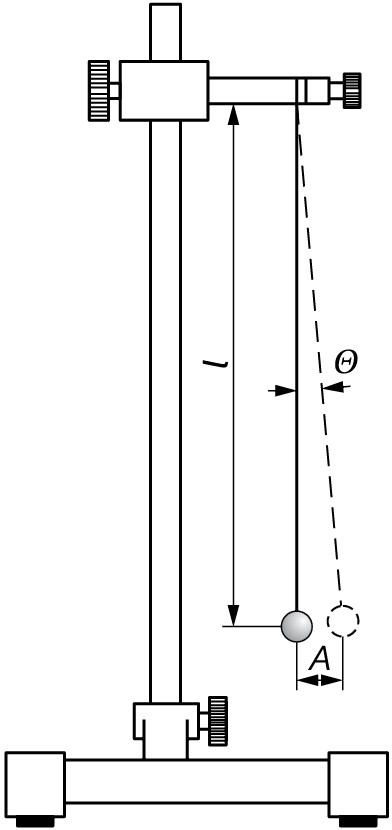
\includegraphics[scale=0.12]{wah.png}
			\caption{Schemat wahadła matematycznego}
			\label{wahadlo}
		\end{figure}
	
%--------------------------------------------------------------------------------------------------------------
	
	\section{Wykonanie ćwiczenia}
	
		\subsection{Pomiary okresu wahadła dla ustalonej długości nici}
			\begin{itemize}
				\item Pomiar długości wahadła od miejsca zaczepienia nici do środka ciężarka za pomocą przymiaru milimetrowego.
				\item Wprowadzenie wahadła w ruch drgający, przy możliwie najmniejszej amplitudzie kątowej 	  z punktu równowagi, w sposób nie wywołujący niechcianego eliptycznego toru ruchu 		  ciężarka.
				\item Wykonanie 10-krotnego pomiaru czasu 20 okresów za pomocą sekundomierza.
				\item Zapisanie wyników do tabeli.
			\end{itemize}
		
		\subsection{Pomiary okresu wahadła dla zmiennej długości nici}
			\begin{itemize}
				\item Pomiar długości wahadła od miejsca zaczepienia nici do środka ciężarka za pomocą 		  przymiaru milimetrowego.
				\item Wprowadzenie wahadła w ruch drgający, przy możliwie najmniejszej amplitudzie kątowej 	  z punktu równowagi, w sposób nie wywołujący niechcianego eliptycznego toru ruchu 		  ciężarka.
				\item Wykonanie 15-krotnego pomiaru czasu 20 okresów wahadła ze zmienną długością nici 	  za pomocą sekundomierza.
				\item Zapisanie wyników do tabeli.
			\end{itemize}
	
%--------------------------------------------------------------------------------------------------------------
	
	\section{Opracowanie danych pomiarowych}
	
	\subsection{Przyspieszenie grawitacyjne dla stałej długości nici wahadła}
	Zmierzone wielkości zapisano w tabeli \ref{Tabela1}, gdzie uwzględniono czas wykonania $k$ okresów w czasie $t$ oraz wyliczono odpowiednią wartość okresu $T$ dla danej próby.
	
	\begin{table}[!h]
		\centering
		\begin{tabular}{ | c | c | c | c | }
			\hline
			\textrm{Lp.} & \textrm{Liczba okresów } k & \textrm{czas } t \textrm{ dla } k \textrm{ okresów [s]} & \textrm{okres } T_i=t/k \textrm{~[s]} \\ \hline
			1 & 20 & 24.8 & 1.240 \\ \hline
			2 & 40 & 49.82 & 1.246 \\ \hline
			3 & 60 & 75.14 & 1.252 \\ \hline
			4 & 80 & 100.11 & 1.251 \\ \hline
			5 & 100 & 125.07 & 1.251 \\ \hline
			6 & 20 & 24.83 & 1.242 \\ \hline
			7 & 40 & 49.89 & 1.247 \\ \hline
			8 & 60 & 74.92 & 1.249 \\ \hline
			9 & 20 & 25.2 & 1.260 \\ \hline
			10 & 40 & 50.23 & 1.256 \\ \hline
		\end{tabular}
		\caption{Pomiar okresu drgań przy ustalonej długości wahadła $l=396$ mm$~\pm~1$ mm.}
		\label{Tabela1}	
	\end{table}

	Z uzyskanych wyników obliczamy wartość średnią:
	
	\begin{equation}
		T_{\textrm{śr}} = \frac{1}{n} \sum_{i = 1}^{n} T_i \approx 1.249
	\end{equation}
	Po podstawieniu uzyskanej wartości do wzoru na przyspieszenie grawitacyjne uzyskujemy:
	
	\begin{equation}
		g = \frac{4 \pi^2 l}{T^2_{\textrm{śr}}} = \frac{4 \cdot (3.141)^2 \cdot 0.396 \textrm{ m}}{(1.249 \textrm{ s})^2} %
		\approx \frac{15.628 \textrm{ m}}{1.561 \textrm{ s}^2} \approx 10.013 ~\frac{\textrm{m}}{\textrm{s}^2}
	\end{equation}
	\label{gStala}
	
	%----------------------------------------------------------------------------------------------------------
	
	\subsection{Przyspieszenie grawitacyjne dla zmiennej długości nici wahadła}
	
	Zbadany okres drgań w zależności od długości wahadła przedstawiono w tabeli \ref{tabela2}.
	
	\begin{table}[!h]
		\centering
		\begin{array}{ | c | c | c | c | c | c | }
			\hline
			\textrm{Lp.} & l \textrm{ [mm]} & k & t \textrm{ [s]} & T \textrm{ [s]} & T^2 \textrm{ [s$^2$]} \\ \hline
			1 & 369 & 20 & 24.8 & 1.240 & 1.538 \\ \hline
			2 & 163 & 20 & 16.31 & 0.816 & 0.665 \\ \hline
			3 & 201 & 20 & 18.06 & 0.903 & 0.815 \\ \hline
			4 & 241 & 10 & 10.1 & 1.010 & 1.020 \\ \hline
			5 & 241 & 20 & 19.91 & 0.996 & 0.991 \\ \hline
			6 & 281 & 30 & 31.97 & 1.066 & 1.136 \\ \hline
			7 & 281 & 20 & 21.38 & 1.069 & 1.143 \\ \hline
			8 & 321 & 20 & 22.75 & 1.138 & 1.294 \\ \hline
			9 & 357 & 10 & 12.09 & 1.209 & 1.462 \\ \hline
			10 & 394 & 10 & 12.54 & 1.254 & 1.573 \\ \hline
			11 & 106 & 10 & 6.63 & 0.663 & 0.440 \\ \hline
			12 & 146 & 10 & 7.82 & 0.782 & 0.612 \\ \hline
			13 & 195 & 10 & 8.94 & 0.894 & 0.799 \\ \hline
			14 & 240 & 10 & 9.85 & 0.985 & 0.970 \\ \hline
			15 & 279 & 10 & 10.69 & 1.069 & 1.143 \\ \hline
		\end{array}
		\caption{Pomiar zależności okresu drgań od długości wahadła $l$}
		\label{tabela2}
	\end{table}

	\begin{figure}[h!]
		\centering
		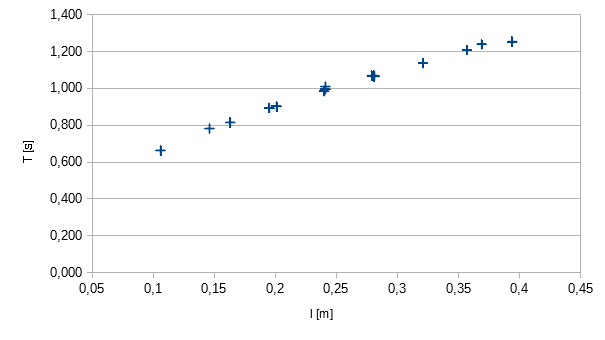
\includegraphics[scale=0.8]{T(l)}
		\caption{Wykres przedstawiający zależność $T(l)$}
		\label{wykr1}
	\end{figure}
	Aby obliczyć przyspieszenie ziemskie posłużymy się krzywą regresji, dlatego przekształcamy wzór (1)	podnosząc obie strony do kwadratu:
	\begin{equation}
		T^2 = \frac{4 \pi^2}{g} l
	\end{equation}
	w ten sposób uzyskaliśmy wzór funkcji liniowej postaci $y = ax + b$, gdzie:
	\begin{equation}
		a = \frac{4 \pi^2}{g}~~,~~b = 0
	\end{equation}
	Możemy teraz stowrzyć wykres $T^2(l)$ oraz za pomocą programu Excel możemy wyznaczyć wzór regresji liniowej.
	\begin{figure}[!h]
		\centering
		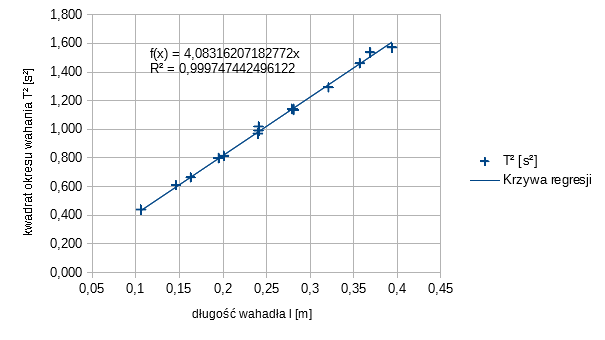
\includegraphics[scale=0.7]{regresja.png}
		\caption{Wykres $T^2(l)$ wraz z zaznaczoną regresją liniową}
	\end{figure}


	Podstawiając $a$ do wzoru funkcji jesteśmy w stanie obliczyć przyspieszenie ziemskie
	\begin{equation}
		g = \frac{4 \pi ^ 2}{a} \approx 9.665 ~\frac{\textrm{m}}{\textrm{s}^2}  
	\end{equation}
	
	%----------------------------------------------------------------------------------------------------------	
	
	\subsection{Analiza niepewności}
	\label{analiza_niepewnosci}
	
	\subsubsection{Niepewność pomiaru długości wahadła}
	Mamy tutaj do czynienia z niepewnością typu B, ponieważ pomiar był wykonywany tylko raz. Znana jest dokładność przymiaru milimetrowego równa działce elementarnej, stąd wnioskujemy że dokładność pomiarów jest równa jej wartości, stąd:
	\begin{equation}
		u(l) = \textrm{działka elementarna} = 0.001 \textrm{ m}
	\end{equation}
	
	\subsubsection{Niepewność pomiaru okresu drgań}
	Z racji, że nie jesteśmy w stanie idealnie zmierzyć czasu trwania jednego okresu drgania przy stałej długości wahadła (czynnik refleksu ludzkiego) zastosujemy tutaj niepewność pomiarową typu A obliczając estymator odchylenia standardowego od średniego okresu
	\begin{equation}
		u(T) = \sqrt{\frac{\sum_{i=1}^{n}(T_i - T_{\textrm{śr}})^2}{n(n-1)}} \approx 0.006 \textrm{ s}
	\end{equation}
	
	\subsubsection{Niepewność złożona wyznaczania przyspieszenia ziemskiego - stała długość}
	Ponieważ nasz pomiar jest złożony z wielu pomiarów obarczonych błędami stosujemy prawo przenoszenia niepewności:
	\begin{equation}
		u_c(g) = \sqrt{\left(\frac{\delta g}{\delta T}\right)^2 u(T)^2 + \left(\frac{\delta g}{\delta l}\right)^2 u(l)^2} \approx 0.099 ~\frac{\textrm{m}}{\textrm{s}^2}
	\end{equation}
	Niepewność należy pomożyć razy $2$ aby uzyskać niepewność na długość przedziału:
	\begin{equation}
	U_c(g) = 2 * u_c(g) \approx 0.199 ~\frac{\textrm{m}}{\textrm{s}^2}
	\end{equation}
	Co wnioskuje wynikiem przyspieszenia ziemskiego dla stałej długości wahadła równą:
	$$ g = (10.013 \pm 0.199) ~\frac{\textrm{m}}{\textrm{s}^2} $$
	Wartość tablicowa przyspieszenia ziemskiego wynosi $g = 9.811 ~\frac{\textrm{m}}{\textrm{s}^2}$ i nieznacznie nie mieści się w przedziale naszego wyniku.
	
	\subsubsection{Niepewność złożona wyznaczania przyspieszenia ziemskiego - zmienna długość}
	Aby oszacować niepewność złożoną pomiaru przyspieszenia ziemskiego dla wahadła o zmiennej długości zastosujemy prawo przenoszenia niepewności dla jednej zmiennej:
	\begin{equation}
		u(g) = \frac{\delta g}{\delta a} u(a) \approx
	\end{equation}
	
%--------------------------------------------------------------------------------------------------------------

	\section{Podsumowanie}

%--------------------------------------------------------------------------------------------------------------
		
\end{document}